\chapter{Results}

In this chapter, we evaluate the performance of the developed adaptive cruise and lane control system via computer simulations. It also briefly explains and discusses some characteristics of the results, whereas a more general discussion follows in the next Chapter. As described in Chapter 4, two agents with different action spaces were investigated. Agent 1 only deals with longitudinal speed control, whereas Agent 2 decides both the speed and when to change lanes.

% Furthermore, two different neural network architectures were used.

%%%%%%%%%%%%%%%%%%%%%%%%%%%%%%%%%%%%%%%%%%%%%%%%%%%%%%%%%%%%%%%%%
\section{Simulation Setup}

In simulations, we used the open source software OpenAI-Gym and ROS / Gazebo which models a highway environment in real time. We generated the environment in order to train the DQN by simulating the behaviors of the cars on highway. In the simulations, we assume that the positions and velocities of the ego vehicle's neighboring vehicles is detected in real time by the ego vehicle. In the beginning of each episode, the position of ego vehicle is set in a defined position but the velocity is initilaized with 0. The initial positions and velocities of other vehicles are initialized based on their lanes. Along with time growing, the relative positions and relative velocities among the vehicles are changing and there have chances to create several different scenarios for the DQN model to learn as below,

\begin{itemize}
\item Scenario 1: No vehicle in the ego vehicle's detecting range.
\item Scenario 2: One vehicle is detected in the same lane of the ego vehicle.
\item Scenario 3: One vehicle is detected but in a different lane of the ego vehicle.
\item Scenario 4: Vehicles are detected in both the ego's lane and the neighboring lane.
\end{itemize}

%%%%%%%%%%%%%%%%%%%%%%%%%%%%%%%%%%%%%%%%%%%%%%%%%%%%%%%%%%%%%%%%%
\section{Training for Single-lane Motion}

The Single-lane Motion means that actions here are all changing the speed. This environment with one lane as shown in Fig. \ref{fig:acc-env} would focus on training an Adaptive Cruise Control agent for the ego vehicle. The ego vehicle and the preceding vehicle would be initialized with defined the positions and headings and surely the relative position is enough safe. The dimension of the state space is set to $n = 3$ and the variables are the velocity of the ego vehicle $v_{ego}$, the longitudinal distance of the vehicles $s_{rel}$ and the relative velocity $v_{rel} = v_{pre} - v_{ego}$. To accelerate the training, they are normalized before feeding to the network.

\begin{figure}[h]
\centering
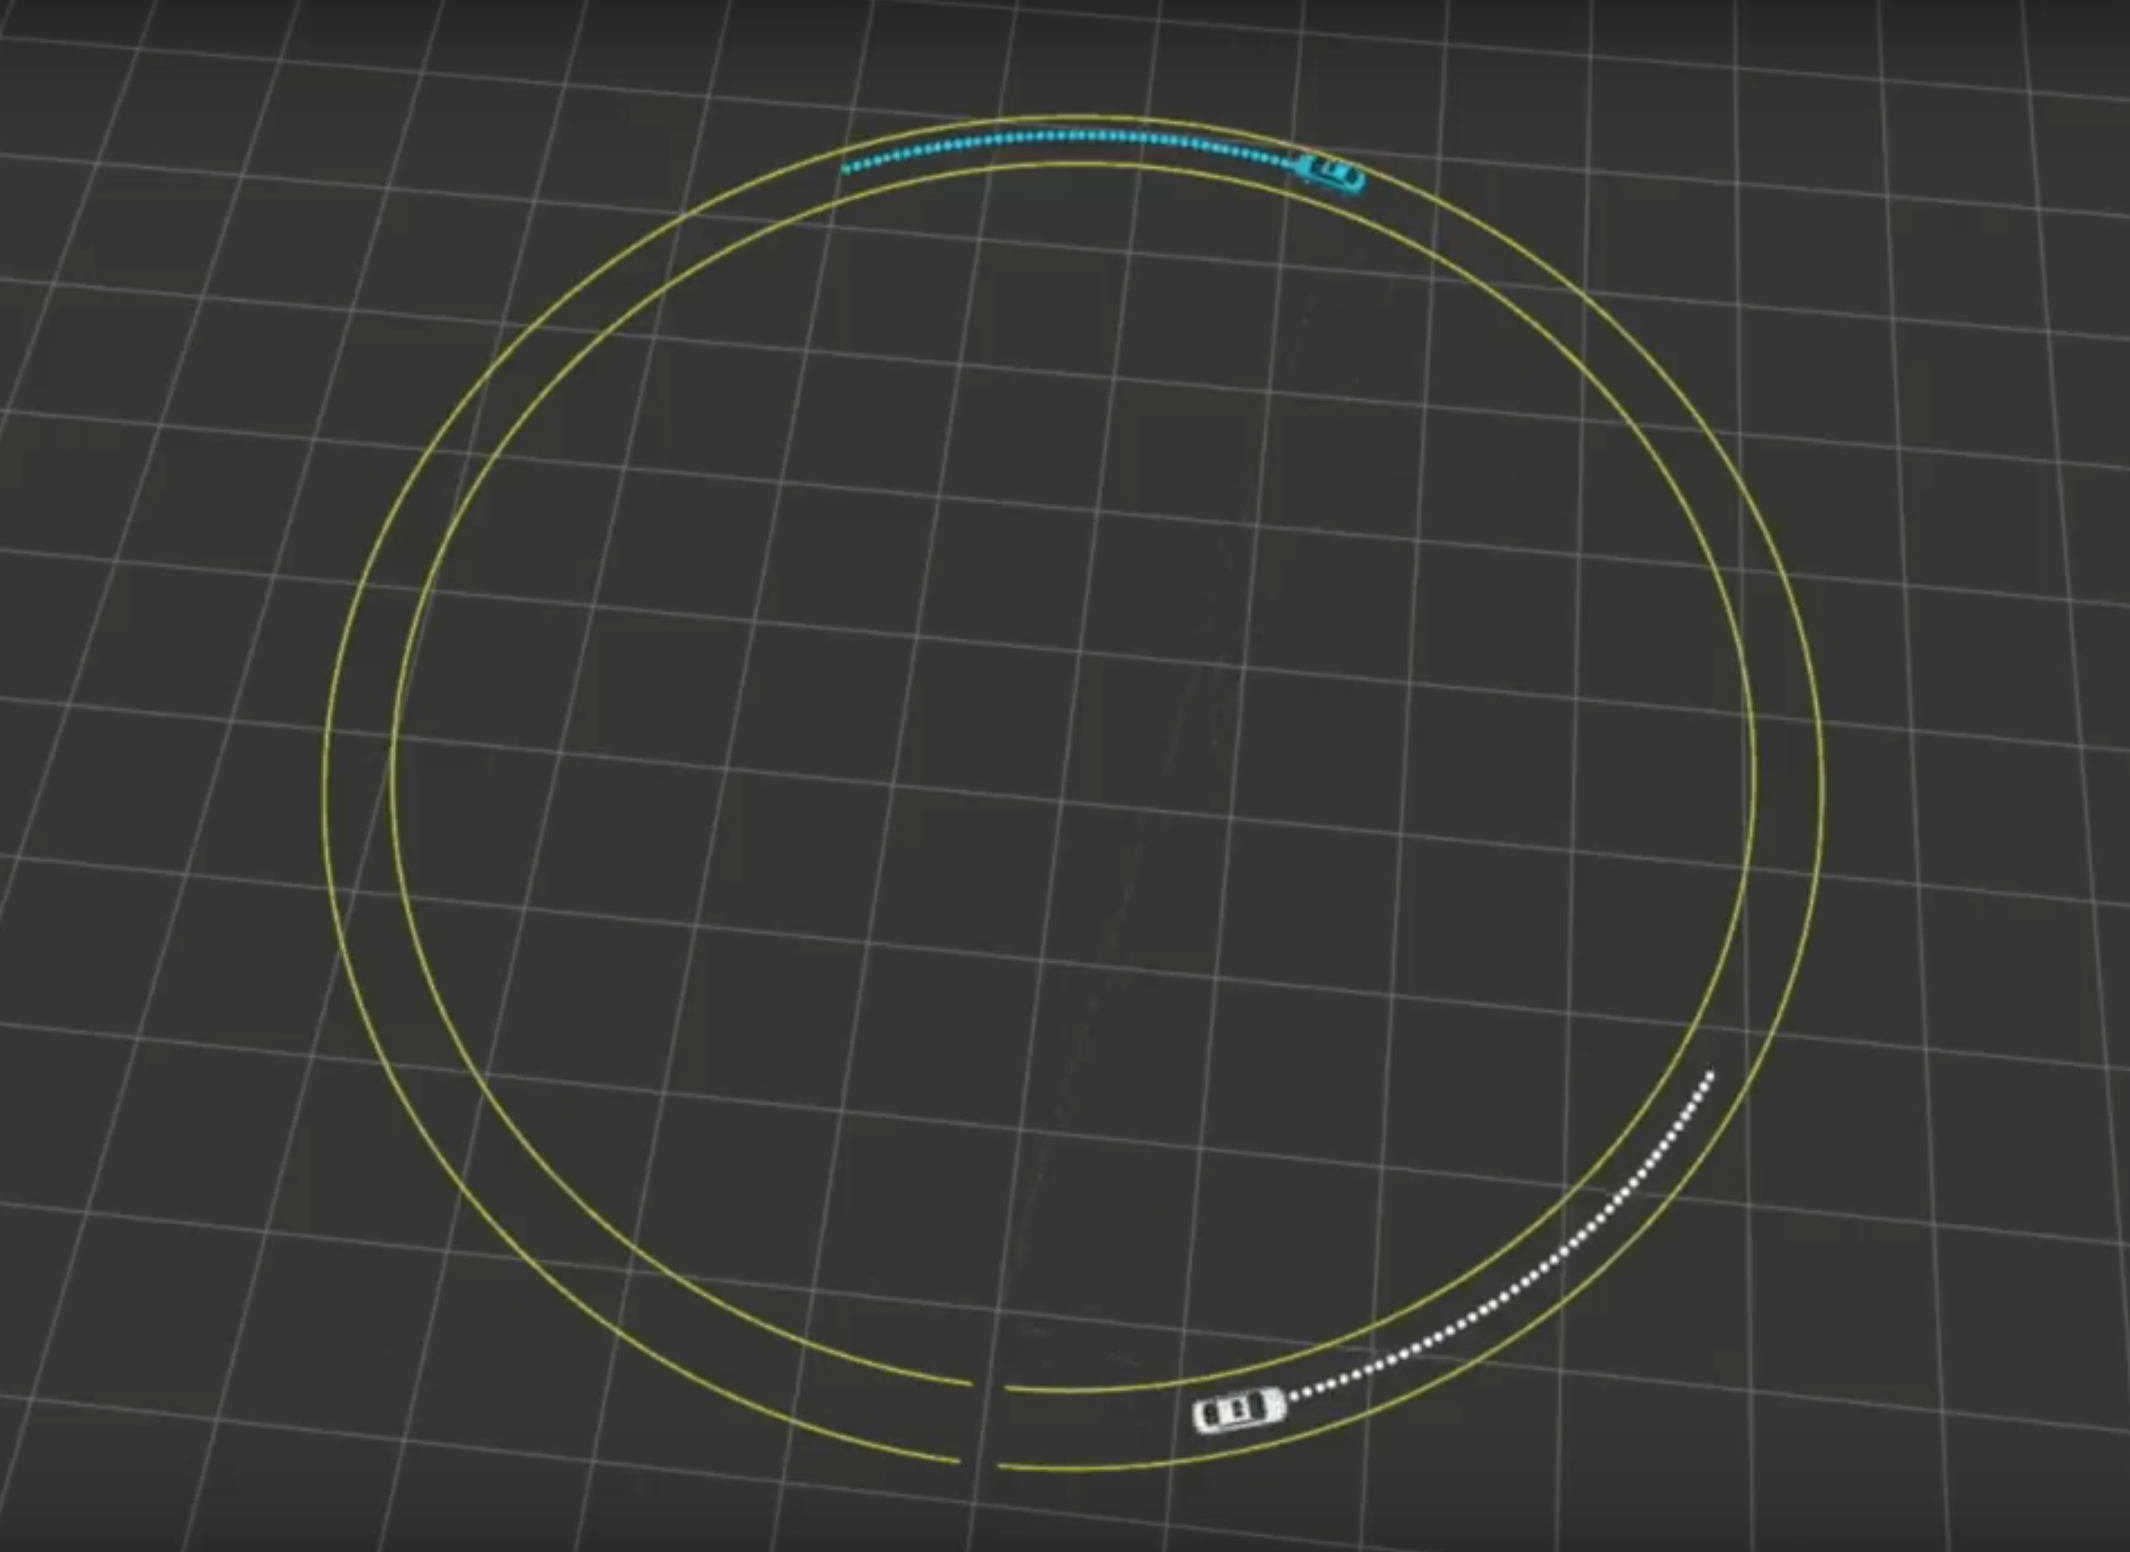
\includegraphics[width=1.0\textwidth]{figs/ch5/acc-env}
\caption{Training environment for Adaptive Cruise Control.}
\label{fig:acc-env}
\end{figure}

The neural network used for the DQN consists of the fully-connected layers with five hidden layers. RMSProp algorithm is used to minimize the loss with learning rate $\epsilon = 0.0005$. We set the size of the replay memory to 10,000. We set the replay batch size to 32. The summary of the DQN configurations used for our experiments is provided below:

\begin{itemize}
\item State buffer size: n = 3
\item Network architecture: fully-connected feed-forward network
\item Nonlinear function: leaky ReLU
\item Number of nodes for each layers : [3 (Input layer), 100, 70, 50, 70, 100, 5 (Output layer)]
\item RMSProp optimizer with learning rate 0.0005
\item Replay memory size: 10,000
\item Replay batch size: 32
\end{itemize}

The parameters are set as below,

\begin{itemize}
\item Cruise speed of the preceding vehicle is $v_{pre} = 10 m/s$ .
\item Safety distance is $dist_{safety} = 10 m$
\item $accel_{high}, accel_{low}, keep_{zero}, decel_{low}, decel_{high} = {2, 1, 0, -1, -2} m/s^2$
\end{itemize}

The reward function is as in Section \ref{eq:reward-func1} and we set $\alpha = 1.0$ and $\beta = 4.0$. 

\begin{itemize}
 \item $r_s$ = incremental travel distance from the last time step (we can simply use euclidean distance between the current position and the previous one since the time is short and curve road can be ignored)
 \item $r_{action}$ = \{accelerate or decelerate with 2 m/s: -1.0, accelerate or decelerate with 1 m/s: -0.5, keep the speed: 0.0\}
 \item $r_{collision}$ = \{No collision: 0.0, Collision: -100\}
\end{itemize}


\begin{figure}[h]
\centering
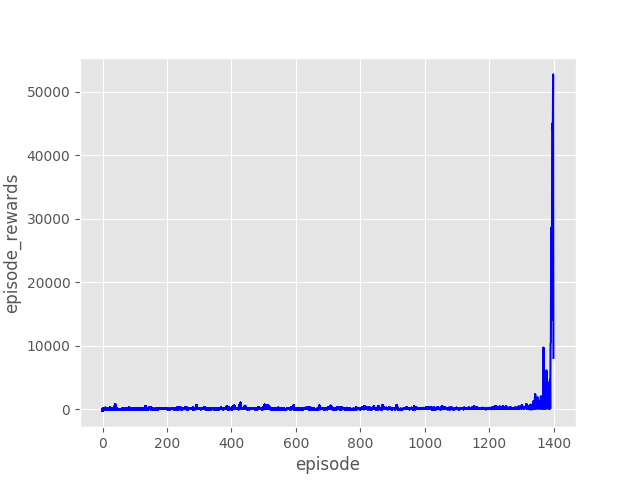
\includegraphics[width=1.0\textwidth]{figs/ch5/acc-reward}
\caption{The reward history of training for Adaptive Cruise Control.}
\label{fig:acc-reward}
\end{figure}

Fig. \ref{fig:acc-reward} provides the plot of the total accumulated rewards i.e., value function achieved for each episode. After 1400 episodes, the plot shows a huge jump in the rewards which means ACC is working and it takes forever to have a collision.

\begin{figure}[h]
\centering
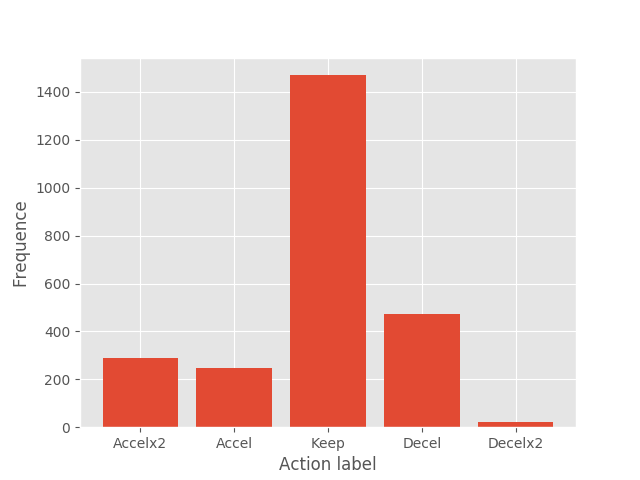
\includegraphics[width=1.0\textwidth]{figs/ch5/acc_action_distribution}
\caption{The action distribution after training.}
\label{fig:acc-action}
\end{figure}

\begin{figure}[h]
\centering
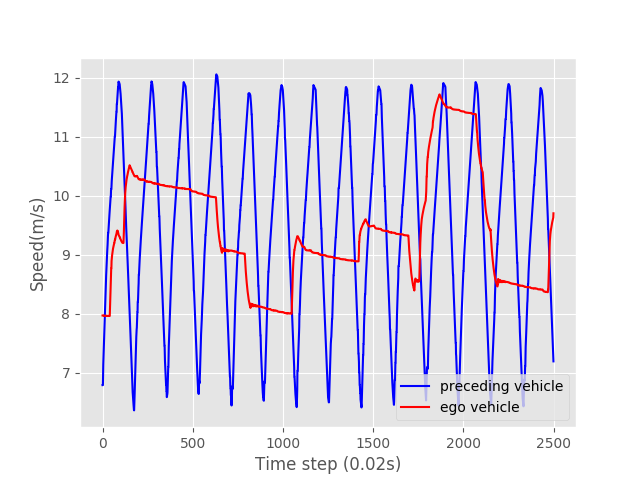
\includegraphics[width=1.0\textwidth]{figs/ch5/vel_variance}
\caption{The speed variance after training.}
\label{fig:acc-vel}
\end{figure}

To quantify the performance after 1400 episodes' training, we recorded a time segment of driving behavior using the trained agent. As shown in Fig. \ref{fig:acc-action}, the actions are mostly chosen as ``Keep the current velocity" since our reward function penalizes any speed changes. About 75\% percent of the actions generated by the agent during the time segment are ``Keep velocity" (labeled as ``2"). Accordingly, the speed variance shown in Fig. \ref{fig:acc-vel} proves that the ego vehicle is closely following the speed of the preceding vehicle. The speed of the preceding vehicle is varying by 2 m/s positively or negatively around 9.5 m/s. The ego vehicle learned to maintain the same average speed but with less variance and it was relatively stable at a speed over multiple time segments, for instance, from $200s$ to $600s$.

%%%%%%%%%%%%%%%%%%%%%%%%%%%%%%%%%%%%%%%%%%%%%%%%%%%%%%%%%%%%%%%%%
\section{Training for Multi-lane Motion}

The Multi-lane Motion means that changing the speed and changing lanes are both available as driving behaviors. This environment with two lanes as shown in Fig. \ref{fig:auto-env} would focus on training an Adaptive Cruise Control and Lane Control agent for the ego vehicle. The ego vehicle and the other two vehicles would be initialized with defined the positions and headings and surely the relative position is enough safe. The dimension of the state space is set to $n = 5$ and the variables are the velocity of the ego vehicle $v_{ego}$, the longitudinal distance of the vehicles $s_{rel}$, the relative velocity $v_{rel} = v_{pre} - v_{ego}$, the flag showing if the left lane is available $flag_{left}$ and the flag showing if the left lane is available $flag_{right}$. To accelerate the training, they are normalized before feeding to the network.

\begin{figure}[h]
\centering
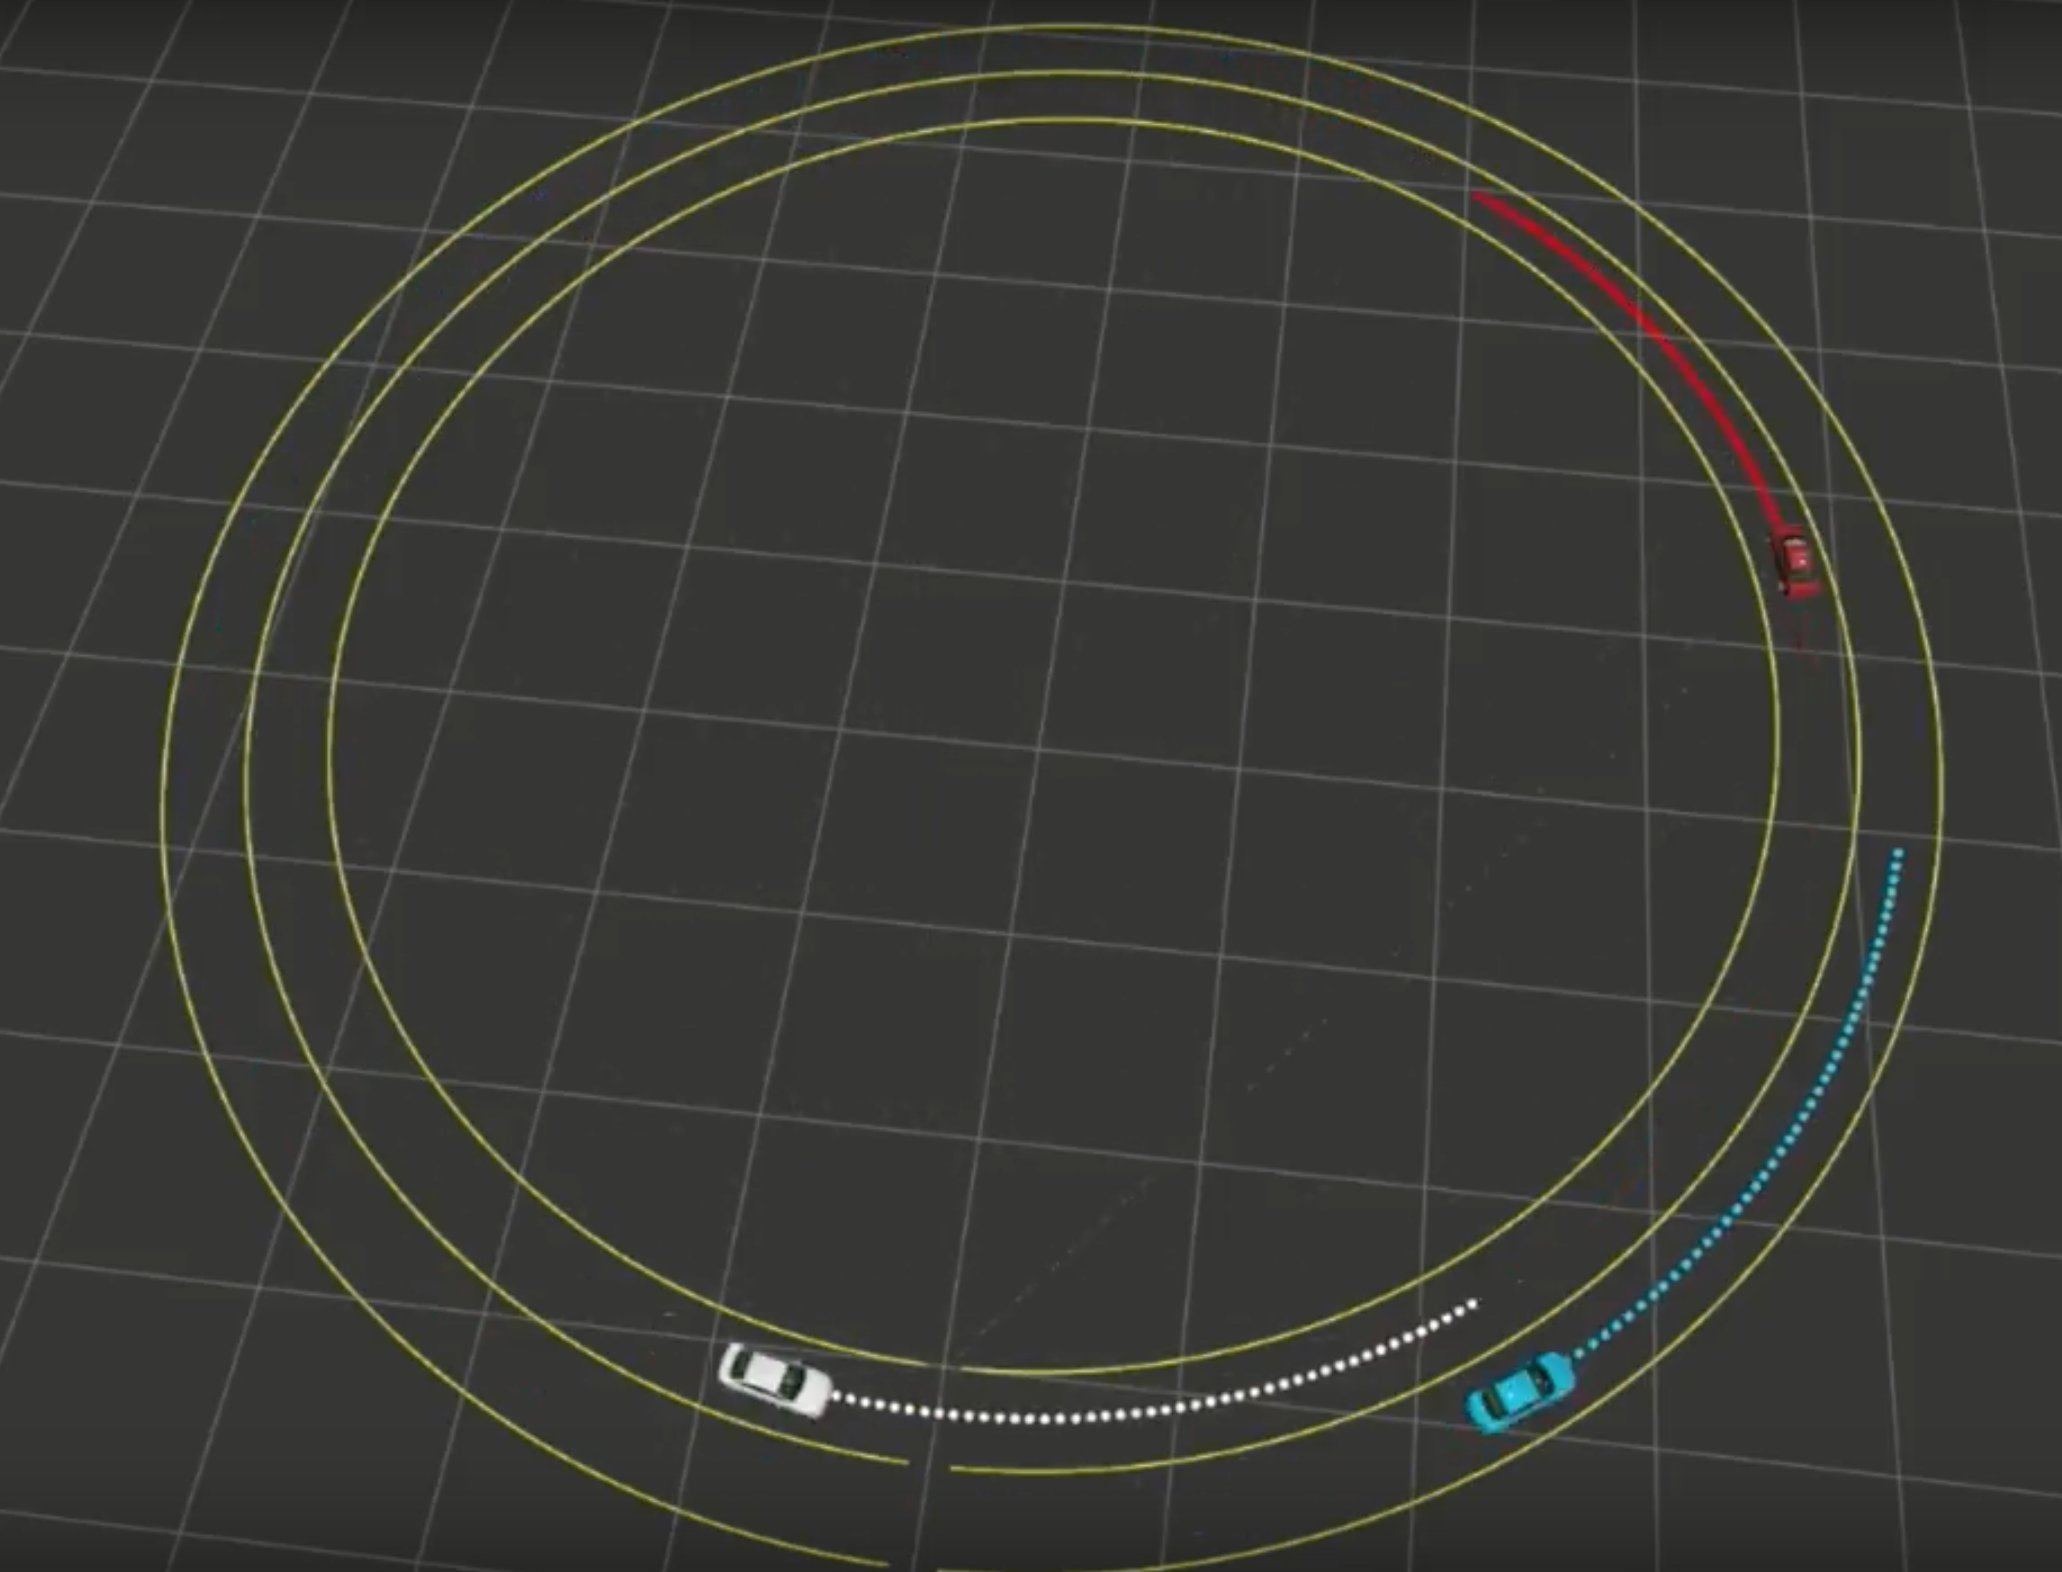
\includegraphics[width=1.0\textwidth]{figs/ch5/auto-env}
\caption{Training environment for Adaptive Cruise Control and Lane Control.}
\label{fig:auto-env}
\end{figure}

The summary of the DQN configurations used for our experiments is provided below:

\begin{itemize}
\item State buffer size: n = 5
\item Action Space size: $7 = 5 + 2$. (5 level of speed control and 2 modes of lane change)
\item Network architecture: fully-connected feed-forward network
\item Nonlinear function: leaky ReLU
\item Number of nodes for each layers : [5 (Input layer), 100, 70, 50, 70, 100, 7 (Output layer)]
\item RMSProp optimizer with learning rate 0.0005
\item Replay memory size: 10,000
\item Replay batch size: 32
\end{itemize}

The parameters are set as below,

\begin{itemize}
\item Cruise speeds in Lane 0 and 1 are $v_{lane0}, v_{lane1}$ = $6 m/s$, $5 m/s$, which means Lane 0 and 2 are Fast Lane and Slow Lane.
\item Safety distance is $dist_{safety} = 10 m$
\item $accel_{high}, accel_{low}, keep_{zero}, decel_{low}, decel_{high}$ = $2 m/s^2$, $1 m/s^2$, $0 m/s^2$, $-1 m/s^2$, $-2 m/s^2$.
\end{itemize}

The reward function is as in Section \ref{eq:reward-func1} and we set $\alpha = 1.0$ and $\beta = 2.0$. 

\begin{itemize}
 \item $r_s$ = travel distance from the last time step (we can simply use euclidean distance between the current position and the previous one since the time is short and curve road can be ignored)
 \item $r_{action}$ = \{accelerate or decelerate with 2 m/s: -1.0, accelerate or decelerate with 1 m/s: -0.5, keep the speed: 0.0, change lane to left or right: -1.0, change lanes when lane is not available: -3.5\}
 \item $r_{collision}$ = \{No collision: 0.0, Collision: -100\}
\end{itemize}

\begin{figure}[h]
\centering
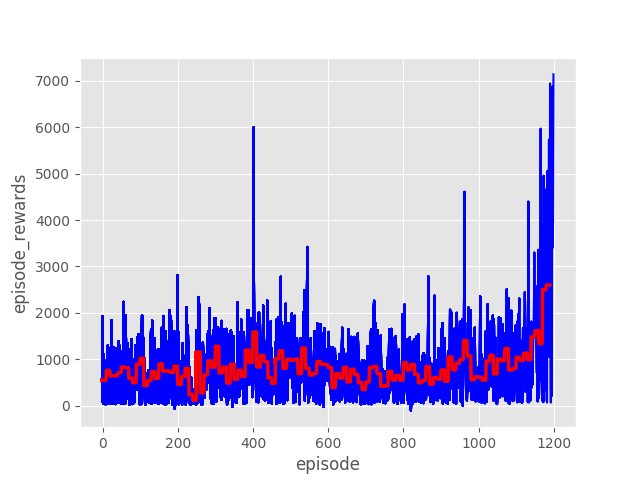
\includegraphics[width=1.0\textwidth]{figs/ch5/auto-reward}
\caption{The reward history of training for Adaptive Cruise Control and Lane Control. (Blue line: the rewards of each time step; Red line: the rewards of every 10 time steps)}
\label{fig:auto}
\end{figure}

Fig. \ref{fig:auto} provides the plot of the total accumulated rewards i.e., value function achieved for each episode. We observe that the reward increases along the episodes and high total reward is attained after 2000 episodes. Until then, the trained agent has enough ability to drive the vehicle safely in multiple lanes using speed control and lane control. Due to the training time limit, more episodes are not provided here. Since it is still exploring the boundaries in the solution space, it has the potential to gain higher rewards with longer training.

\begin{figure}[h]
\centering
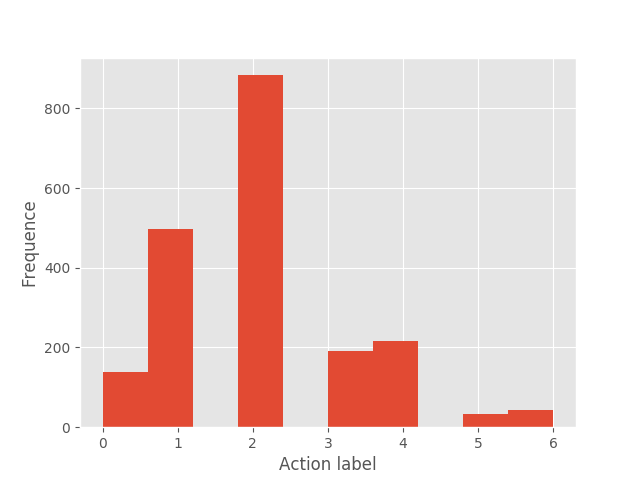
\includegraphics[width=1.0\textwidth]{figs/ch5/auto_action_distribution}
\caption{The action distribution after training.}
\label{fig:auto-action}
\end{figure}

\begin{figure}[h]
\centering
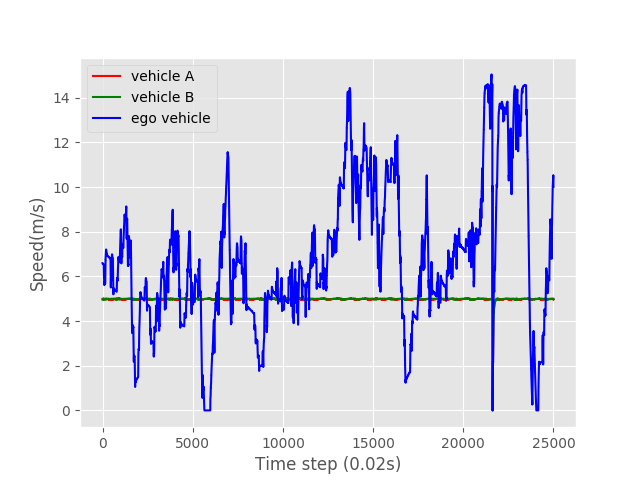
\includegraphics[width=1.0\textwidth]{figs/ch5/auto_vel}
\caption{The speed variance after training.}
\label{fig:auto-vel}
\end{figure}

Fig. \ref{fig:auto-action} shows the action distribution after training. Most times it will stay at constant speed by action ``Keep speed" (labeled as ``2"). The agent will rarely choose to change lanes since it would be always safe to stay in the current lane as long as the ACC is reliable. Sometimes it would try to change lanes and accelerate (labeled as ``0" and ``1") when no vehicle is ahead in the new lane. 

As shown in Fig. \ref{fig:auto-vel}, the speed varied to a higher degree than that in Fig. \ref{fig:acc-vel}. That is because when lane change is available or the action space is bigger the agent takes more time to make decisions and is more likely to make mistakes. Overall, it learned to maintain an equal average speed with the preceding vehicle and accelerate when changing to a new lane when there is no vehicle right ahead. With more time training, it could be expected to perform better.

\section{Main Evaluation}

Both $Agent1_{FCNN}$ and $Agent2_{FCNN}$ successfully drove the ego vehicle safely without collisions for a very long time and distance after enough training. Naturally, $Agent1_{FCNN}$ solved a significantly higher fraction of the episodes and performed better than $Agent2_{FCNN}$, since it only needed to control the speed, and not decide when to change lanes. In the beginning, $Agent1_{FCNN}$ learned to always stay in its position to avoid an immediate collision, but quickly met a limit in receiving higher reward. With more training, it started to maintain a relatively high speed and keep stable if a preceding vehicle was detected, but sometimes caused collisions. $Agent2_{FCNN}$ needs much more training to stay safe. A longer training run could be carried out for better performance.

Between the two, the ACC agent is of the key importance which makes the vehicle safe. Lane control is to optimize the driving behavior. Especially we show long run performance here to validate the ACC agent. Later in Chapter 6, two video of the two agents would be provided to show the trained behaviors intuitively.

 \begin{figure}[h]
\centering
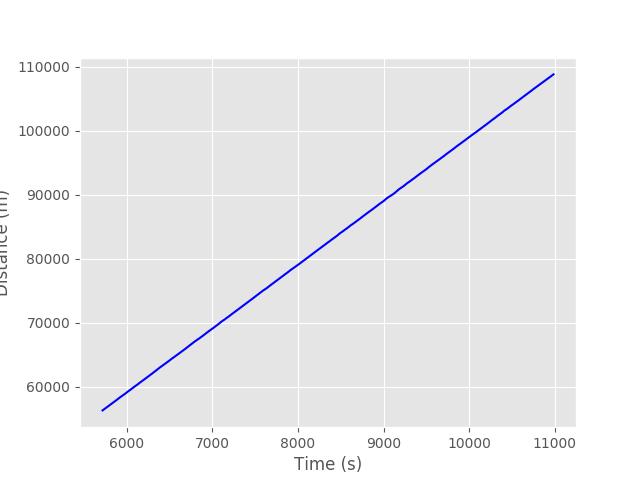
\includegraphics[width=0.8\textwidth]{figs/ch5/long_distance_variance}
\caption{The distance variance with time in a long run.}
\label{fig:long_distance_variance}
\end{figure}

\begin{figure}[h]
\centering
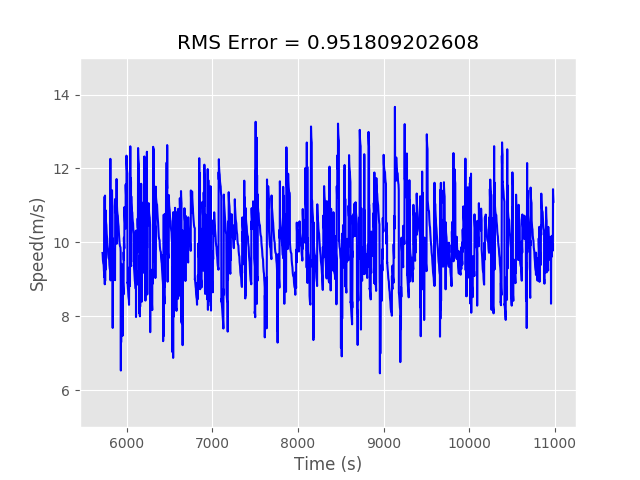
\includegraphics[width=0.8\textwidth]{figs/ch5/long_speed_variance}
\caption{The speed variance with time in a long run.}
\label{fig:long_speed_variance}
\end{figure}

\begin{figure}[h]
\centering
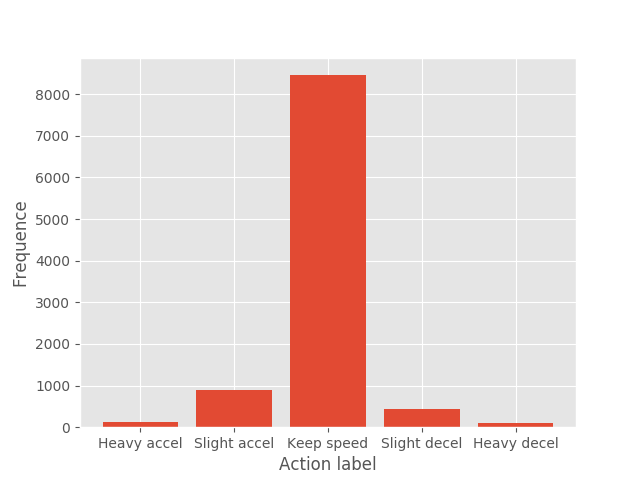
\includegraphics[width=0.8\textwidth]{figs/ch5/long_travel_action}
\caption{The action frequency in a long run.}
\label{fig:long_travel_action}
\end{figure}

The leading vehicle is following a sine curve in the ACC training stage. The extreme setting is required to train the agent to have better adaptive ability in unstable scenarios. What if the preceding vehicle is at a stable speed which is more common in real life. We can use a vehicle with a constant speed like 10 meters per second to test the ACC agent and run several hours. The performance would be valued by how smooth the speed varies, how far the ego vehicle safely drive and how stable in choosing actions.

The three figures, Fig. \ref{fig:long_distance_variance}, Fig. \ref{fig:long_speed_variance} and Fig. \ref{fig:long_travel_action}, show the performance in a more general and longer run. 

\begin{itemize}
	\item \textbf{Persistence.} The agent is able to drive the vehicle continuously within 10000 time steps (also 10000 seconds) which is the upper limit in my setting. It can travel 100,000 meters with an average speed 10 m/s.
	\item \textbf{Speed Variance.} The speed is oscillating around the average line as shown in Fig. \ref{fig:long_speed_variance}, though it is smooth in Fig. \ref{fig:long_distance_variance}. The Root Mean Square Error (RMSE) of the actual speed with a constant 10 m/s line is computed as 0.95 which can be lowered by tuning the reward function.
	\item \textbf{Behavior Selecting.} Behavior selecting or action choosing has been optimized as expected in the reward function design. Fig. \ref{fig:long_travel_action} records from Time step 0 to Time step 9999, the actions converge to "Keep" (namely Keep the speed) which have about 85\% in all.
\end{itemize}


